%%%%%%%%%%%%%%%%%%%%%%%%%%%%%%%%%%
% ICRA 2018 Submission Manuscript
% John Romanishin, John Mamish, and Daniela Rus
% SEPTEMBER 2017
%%%%%%%%%%%%%%%%%%%%%%%%%%%%%%%%%% 
     
\documentclass[letterpaper, 10 pt, conference]{ieeeconf}  
\IEEEoverridecommandlockouts  % This command is only needed if you
			      % want to use the \thanks command
\overrideIEEEmargins
% See the \addtolength command later in the file to balance the column lengths on the last page of the document
\ifx\pdfoutput\undefined

%%%%%%%%%%%%%%%
%%%      Packages       %%%
%%%%%%%%%%%%%%%

% we are running LaTeX, not pdflatex
\usepackage[dvips]{graphicx}
\else
% we are running pdflatex, so convert .eps files to .pdf
\usepackage[pdftex]{graphicx}
\usepackage{epstopdf}
\fi

\usepackage{amsmath, amssymb, mathptmx}
\usepackage{algorithmic}
\usepackage{algorithm}
\usepackage{multirow}
\usepackage{breakurl}
\usepackage{caption}
\usepackage{subcaption}
\usepackage[bookmarks=true,breaklinks=true,]{hyperref}
\newtheorem{theorem}{Theorem}

%%%  	 TIKZ 	  %%%

\usepackage{pgfplots}
\usetikzlibrary{math} %needed tikz library
\usepackage{tikz-dimline}
\usepackage{tikz}
\usetikzlibrary{arrows,shapes,trees}
\usetikzlibrary{calc,trees,positioning,arrows,chains,shapes.geometric,%
decorations.pathreplacing,decorations.pathmorphing,shapes,%
matrix,shapes.symbols,plotmarks,decorations.markings,shadows,arrows.meta,bending}
\definecolor{maroon}{RGB}{111,0,15}
\definecolor{light_orange}{RGB}{150,100,50}


%%%%%%%%%%%%%%%
%%%      Packages       %%%
%%%%%%%%%%%%%%%
\newcommand{\hvectspace}{\hspace{.2cm}}

\title{\LARGE \bf Mblocks Stigmergic Tags and Algorithims}

\author{John W. Romanishin, John Mamish, and Daniela Rus
  \thanks{J. W. Romanishin, D. Rus are with the Computer Science
    and Artificial Intelligence Lab, MIT, Cambridge, MA, 02139
    {\tt\small \{johnrom|rus\}@csail.mit.edu}.}
}

\begin{document}
	
\newcommand{\tagName}{mtag }
\newcommand{\tagNamePlural}{mtags }

\captionsetup[figure]{labelfont=small, textfont=small}
\captionsetup[table]{labelfont=small, textfont=small}

\maketitle

\thispagestyle{empty}
\pagestyle{empty}

%%%%%%%%%%%%%%%%%%
\begin{abstract}
%%%%%%%%%%%%%%%%%% 

This paper presents distributed algorithms which utilize a novel type of magnetic barcode and mesh wireless networks to guide the reconfiguration of 3D M-Blocks modular robotic modules. The 3D Mblocks modular robots, original described in ~\cite{RomanishinRus-IROS13} and ~\cite{RomanishinRus-IROS13} have been outfitted with a novel type of magnetic tag and reader circuitry on each face, so that modules can accurately read ID information for other modules, or messages encoded in specially signified tags in the environment. This ability allows for a scalable, reliable, inexpensive, and simple way to identify their location information.

%%%%%%%%%%%%%%%%%%
\end{abstract}
%%%%%%%%%%%%%%%%%%

%%%%%%%%%%%%%%%%%%%%%%%%%
\section{Introduction}
\label{sec:Introduction}
%%%%%%%%%%%%%%%%%%%%%%%%%

Modular Self-Reconfigurable Robots (MSRR) have been proposed as one method to create general purpose robotic systems of arbitrary complexity in an autonomous way. MSRR systems generally can be thought of as consisting of individual \emph{modules}, which connect to either other active modules or passive modular elements, through standardized \emph{connectors} to create a specific \emph{configuration} in order to accomplish a designated task. Much of the work in the MSRR field has focused either on the preliminary development of novel hardware systems, or general purpose algorithms on simulated systems. Few MSRR systems have remained under active development long enough in order to develop practical algorithms that can accomplish tasks using actual hardware. This paper is focused on implementing and analyzing three separate practical partially decentralized "behaviors" with a set of 3D M-Block modules.

\newsavebox{\arrows}
\sbox{\arrows}
{
	\resizebox{1.4 in}{!}
	{
	\begin{tikzpicture}[x=(220:1cm), y=(-40:1cm), z=(90:0.707cm)]
		%%
%this code is from...
\setcounter{x}{0}%
\setcounter{y}{0}%
\setcounter{z}{0}%

% The angles of x,y,z-axes
\newcommand\xaxis{210}
\newcommand\yaxis{-30}
\newcommand\zaxis{90}

% The top side of a cube
\newcommand\topside[3]{
	\fill[fill=yellow, draw=black,shift={(\xaxis:#1)},shift={(\yaxis:#2)},
	shift={(\zaxis:#3)}] (0,0) -- (30:1) -- (0,1) --(150:1)--(0,0);
}

% The left side of a cube
\newcommand\leftside[3]{
	\fill[fill=red, draw=black,shift={(\xaxis:#1)},shift={(\yaxis:#2)},
	shift={(\zaxis:#3)}] (0,0) -- (0,-1) -- (210:1) --(150:1)--(0,0);
}

% The right side of a cube
\newcommand\rightside[3]{
	\fill[fill=blue, draw=black,shift={(\xaxis:#1)},shift={(\yaxis:#2)},
	shift={(\zaxis:#3)}] (0,0) -- (30:1) -- (-30:1) --(0,-1)--(0,0);
}

% The cube 
\newcommand\cube[3]{
	\topside{#1}{#2}{#3} \leftside{#1}{#2}{#3} \rightside{#1}{#2}{#3}
}

\newcommand\ArrowNE[3]
{
	\node at (#1+0.5, #2+0.5, #3) 
%	\node at (#1, #2, #3) 
	{
		\begin{tikzpicture}
		\draw[->, thick, >={Stealth[round]}, line width=0.4mm] (0.3,0) -- (-0.3,0);
		\end{tikzpicture}};
		
}

\newcommand\ArrowNL[3]
{
	\node at (#1+1, #2+0.5, #3-0.5) 
	%	\node at (#1, #2, #3) 
	{
		
\begin{tikzpicture}
		\draw[->, thick, >={Stealth[round]}, line width=0.4mm] (0.16,0.16) -- (-0.16,-0.16);
		\end{tikzpicture}};
	
}

\newcommand\ArrowNR[3]
{
	\node at (#1+0.5, #2+1, #3-0.5) 
	%	\node at (#1, #2, #3) 
	{
		
\begin{tikzpicture}
		\draw[->, thick, >={Stealth[round]}, line width=0.4mm] (0.16,0.16) -- (-0.16,-0.16);
		\end{tikzpicture}};
	
}

\newcommand\ArrowNW[3]
{
	\node at (#1+0.5, #2+0.5, #3) 
%	\node at (#1, #2, #3) 
	{
		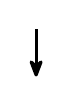
\begin{tikzpicture}
		\draw[->, thick, >={Stealth[round]}, line width=0.4mm] (0,0.3) -- (0,-0.3);
		\end{tikzpicture}};
	
}

\newcommand\ArrowSW[3]
{
	\node at (#1+0.5, #2+0.5, #3) 
%	\node at (#1, #2, #3) 
	{
		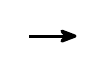
\begin{tikzpicture}
		\draw[<-, thick, >={Stealth[round]}, line width=0.4mm] (0.3,0) -- (-0.3,0);
		\end{tikzpicture}};
	
}

\newcommand\ArrowSE[3]
{
	\node at (#1+0.5, #2+0.5, #3) 
%	\node at (#1, #2, #3) 
	{
		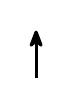
\begin{tikzpicture}
		\draw[<-, thick, >={Stealth[round]}, line width=0.4mm] (0,0.3) -- (0,-0.3);
		\end{tikzpicture}};
	
}

% Definition of \planepartition
% To draw the following plane partition, just write \planepartition{ {a, b, c}, {d,e} }.
%  a b c
%  d e
\newcommand\planepartition[1]{
	\setcounter{x}{-1}
	\foreach \a in {#1} {
		\addtocounter{x}{1}
		\setcounter{y}{-1}
		\foreach \b in \a {
			\addtocounter{y}{1}
			\setcounter{z}{-1}
			\foreach \c in {0,...,\b} {
				\addtocounter{z}{1}
				\ifthenelse{\c=0}{\setcounter{z}{-1},\addtocounter{y}{0}}{
					\cube{\value{x}}{\value{y}}{\value{z}}}
			}
		}
	}
}


%%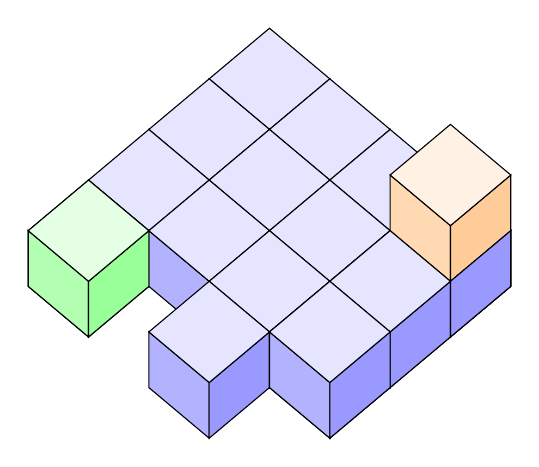
\begin{tikzpicture}[x=(220:1cm), y=(-40:1cm), z=(90:0.707cm)]
	%\planepartition{{0,0,1},{1,1,1},{1,0,0},{1,0,1}};
\foreach \m [count=\y] in {{1,1,1,1},{1,1,1},{1,1,1,1},{1,1,1}}{
	\foreach \n [count=\x] in \m {
		\ifnum \n>0
		\foreach \z in {1,...,\n}{
			\draw [fill=blue!30] (\x+1,\y,\z) -- (\x+1,\y+1,\z) -- (\x+1, \y+1, \z-1) -- (\x+1, \y, \z-1) -- cycle;
			\draw [fill=blue!40] (\x,\y+1,\z) -- (\x+1,\y+1,\z) -- (\x+1, \y+1, \z-1) -- (\x, \y+1, \z-1) -- cycle;
			\draw [fill=blue!10] (\x,\y,\z)   -- (\x+1,\y,\z)   -- (\x+1, \y+1, \z)   -- (\x, \y+1, \z) -- cycle;  
		}
	
		\fi
	}
}   

\foreach \m [count=\y] in {{0,0,0,1}, {0,0,0}} {
	\foreach \n [count=\x] in \m {
		\ifnum \n>0
		\foreach \z in {1,...,\n}{
			\draw [fill=green!30] (\x+1,\y,\z) -- (\x+1,\y+1,\z) -- (\x+1, \y+1, \z-1) -- (\x+1, \y, \z-1) -- cycle;
			\draw [fill=green!40] (\x,\y+1,\z) -- (\x+1,\y+1,\z) -- (\x+1, \y+1, \z-1) -- (\x, \y+1, \z-1) -- cycle;
			\draw [fill=green!10] (\x,\y,\z)   -- (\x+1,\y,\z)   -- (\x+1, \y+1, \z)   -- (\x, \y+1, \z) -- cycle;  
		}
		
		\fi
	}
}   

\ArrowNW{1}	{3}	{1};

\foreach \m [count=\y] in {{0,0,0,0},{0,0,0},{0,0,0,0},{2,0,0}}{
	\foreach \n [count=\x] in \m {
		\ifnum \n>0
		\foreach \z in {1,...,\n}{
			\draw [fill=orange!30] (\x+1,\y,\z) -- (\x+1,\y+1,\z) -- (\x+1, \y+1, \z-1) -- (\x+1, \y, \z-1) -- cycle;
			\draw [fill=orange!40] (\x,\y+1,\z) -- (\x+1,\y+1,\z) -- (\x+1, \y+1, \z-1) -- (\x, \y+1, \z-1) -- cycle;
			\draw [fill=orange!10] (\x,\y,\z)   -- (\x+1,\y,\z)   -- (\x+1, \y+1, \z)   -- (\x, \y+1, \z) -- cycle;  
		}
		
		\fi
	}
}  

\foreach \m [count=\y] in {{0},{0},{0},{0,1,1}}{
	\foreach \n [count=\x] in \m {
		\ifnum \n>0
		\foreach \z in {1,...,\n}{
			\draw [fill=blue!30] (\x+1,\y,\z) -- (\x+1,\y+1,\z) -- (\x+1, \y+1, \z-1) -- (\x+1, \y, \z-1) -- cycle;
			\draw [fill=blue!40] (\x,\y+1,\z) -- (\x+1,\y+1,\z) -- (\x+1, \y+1, \z-1) -- (\x, \y+1, \z-1) -- cycle;
			\draw [fill=blue!10] (\x,\y,\z)   -- (\x+1,\y,\z)   -- (\x+1, \y+1, \z)   -- (\x, \y+1, \z) -- cycle;  
		}
		
		\fi
	}
} 

\foreach \m [count=\y] in {{0},{0},{0},{1,0,0}}{
	\foreach \n [count=\x] in \m {
		\ifnum \n>0
		\foreach \z in {1,...,\n}{
		%	\draw [fill=blue!30] (\x+1,\y,\z) -- (\x+1,\y+1,\z) -- (\x+1, \y+1, \z-1) -- (\x+1, \y, \z-1) -- cycle;
			\draw [fill=blue!40] (\x,\y+1,\z) -- (\x+1,\y+1,\z) -- (\x+1, \y+1, \z-1) -- (\x, \y+1, \z-1) -- cycle;
		%	\draw [fill=blue!10] (\x,\y,\z)   -- (\x+1,\y,\z)   -- (\x+1, \y+1, \z)   -- (\x, \y+1, \z) -- cycle;  
		}
		
		\fi
	}
} 
		"x" "y" "z"

\ArrowNR{4} {1}	{1};
\ArrowNL{4} {1}	{1};

\ArrowNR{4} {3}	{1};
\ArrowNL{4} {3}	{1};

\ArrowNR{3} {4}	{1};
\ArrowNL{3} {4}	{1};

\ArrowNR{1} {4}	{1};
\ArrowNR{2} {4}	{1};

\ArrowNL{3} {2}	{1};

\ArrowSW{1}	{1}	{1};
\ArrowSW{2}	{1}	{1};
\ArrowSW{3}	{1}	{1};
\ArrowSW{4}	{1}	{1};


\ArrowNW{1}	{2}	{1};
\ArrowSW{2}	{2}	{1};
\ArrowNW{3}	{2}	{1};

\ArrowNW{2}	{3}	{1};
\ArrowNE{3}	{3}	{1};
\ArrowNE{4}	{3}	{1};

%\ArrowNW{1}	{4}	{1};
\ArrowSW{2}	{4}	{1};
\ArrowNW{3}	{4}	{1};
;
	\end{tikzpicture}
	}
}

\begin{figure}[t]
	\centering
	\begin{subfigure}[b]{1.6 in}
		%	\resizebox{.48\linewidth}{0.6 in}
		%	{
		\begin{tikzpicture}[]	
		\node at (0,0) {\includegraphics[width=.9\linewidth]{Figures/mTagsCover.png}};
		\node[opacity = 0.95, fill = white, rounded corners] at (-1.45,-1) {(a)};
		\end{tikzpicture}
		
		%	}
		%\subcaption{}
	\end{subfigure}
	~
	\begin{subfigure}[b]{0.48\linewidth}
	%	\resizebox{\linewidth}{!}
	%	{
		\begin{tikzpicture}[]
			\node at (0 cm, 0cm) {\usebox{\arrows}};
			\node[opacity = 0.95, fill = white, rounded corners] at (-1.5,-1.25) {(b)};
		\end{tikzpicture}
	%	}
	\end{subfigure}

	\begin{subfigure}[b]{\linewidth}
		\centering
		\begin{tikzpicture}[]	
		\node at (0,0) {\includegraphics[width=.96\linewidth]{figures/ActualLine_3_small.png}};
		\node[opacity = 0.95, fill = white, rounded corners] at (-3.5,-1.75) {(c)};
		\end{tikzpicture}

	\end{subfigure}
	
	
	\caption{This figure shows a sample of several behaviors implemented with the 3D M-Blocks robots. (a) Shows a photo of an active module connected to a passive module which contains a Magnetic Fiducial. (b) Demonstrates an abstraction of these embedded commands as "arrows" which a module that is attempting to follow a path would move along. In this example, the module shown in \emph{orange} would arrive at the \emph{green} module after successfully implementing the path following behavior. (c) Shows several modules implementing the line formation behavior.}
	
	\label{fig:intro}
\end{figure}

The conceptually simplest framework for controlling thousands or millions of individual modular robots is to have a centralized authority which dictates every move to each robot. However these systems suffer from practical problems maintaining the required number of communication links and a general lack of robustness to disturbances. One approach is to develop embedded "behaviors" or simple decentralized algorithms which each module can implement independently in the (potentially temporary) absence of centralized commutations. When developing these behaviors, the type of sensor feedback, and (un)availability and type of local communication are important to determining the possible complexity of these behaviors. This work focuses on modules which have information only about their direct neighbors, global input from a stimulus source (i.e. visible light), knowledge about gravity, and occasional wireless communication with a higher level controller. The behaviors that we introduce include (1) Path following, (2) Line formation, and (3) Light guided aggregation. The ability for MSRR systems to delegate most of the detailed movements to be autonomously handled by individual modules based on local interactions, while still able to assert control when necessary improves the scalability of the system. While there have been similar proposed decentralized control strategies, several of which are discussed in Section~\ref{ssec:RW-Algorithmic}, this work focuses on defining and adapting these behaviors for an existing robotic platform.

This work is implemented and experimentally validated through a set of twelve 3D M-Block modular robots; which are one of the few MSRR systems capable of three-dimensional reconfiguration according to a generalized 3D lattice reconfiguration model. These 50~mm cubic modules use pulses of angular momentum and temporary magnetic hinges in order to implement lattice reconfiguration according to the Pivoting Cube Model (PCM). The M-Blocks were introduced for 2D movement in 2013~\cite{RomanishinRus-IROS13} and extended to three dimensions in 2015~\cite{Romanishin20153d}. In order to facilitate the implementation of new primitive behaviors, the 3D M-Blocks are further extended in this work to include a novel type of magnetic fiducial which allows modules to detect information about their neighbors. These new fiducial tags, called \tagNamePlural, provides globally unique identification codes for each face of a collection of modules. \TagNamePlural~include relative orientation of the connection between the reading module, and are completely passive, allowing the system to accurately determine its global configuration even when various modules are either disabled or are passive elements.

Specifically this paper presents the following technical contributions:
\begin{itemize}
	\item Developed and characterized a new type of magnetic fiducial (\TagNamePlural) specifically designed to address the task of neighbor identification and determining connection orientation for MSRR. (Section~\ref{sec:Hardware})
	\item Defined three separate primitive MSRR behaviors (distributed algorithms), tailored for the 3D M-Block hardware system. (Section~\ref{sec:Behaviors})
	\item Experimentally validated these behaviors on a system of twelve 3D M-Block modules. (Section~\ref{sec:Experiments})
\end{itemize}

%The remainder of the paper is organized as follows: Section~\ref{sec:RelatedWork} gives an overview of related work that pertains to modular robots with a focus on how existing %MSRR systems identify and encode physical configuration information through their connectors. Next, Section~\ref{sec:Hardware} presents the technical details of the proposed %\tagNamePlural~system for determining neighbor connection information and then attempts to characterize their functionality and discusses current limitations and potential %future extensions. Next, Section ~\ref{sec:Behaviors} presents the detailed algorithms which implement the three behaviors, (1) Path following: (2) Line formation and (3) Light %Aggregation, while Section~\ref{sec:Experiments} presents and analyzes experiments implementing these three algorithms. Finally, Section~\ref{sec:Discussion} attempts to help %illustrate several of the challenges and requirements for eventually applying these behaviors to future systems with millions of modules.


%\begin{figure}[htb]
%
%	%%
%this code is from...
\setcounter{x}{0}%
\setcounter{y}{0}%
\setcounter{z}{0}%

% The angles of x,y,z-axes
\newcommand\xaxis{210}
\newcommand\yaxis{-30}
\newcommand\zaxis{90}

% The top side of a cube
\newcommand\topside[3]{
	\fill[fill=yellow, draw=black,shift={(\xaxis:#1)},shift={(\yaxis:#2)},
	shift={(\zaxis:#3)}] (0,0) -- (30:1) -- (0,1) --(150:1)--(0,0);
}

% The left side of a cube
\newcommand\leftside[3]{
	\fill[fill=red, draw=black,shift={(\xaxis:#1)},shift={(\yaxis:#2)},
	shift={(\zaxis:#3)}] (0,0) -- (0,-1) -- (210:1) --(150:1)--(0,0);
}

% The right side of a cube
\newcommand\rightside[3]{
	\fill[fill=blue, draw=black,shift={(\xaxis:#1)},shift={(\yaxis:#2)},
	shift={(\zaxis:#3)}] (0,0) -- (30:1) -- (-30:1) --(0,-1)--(0,0);
}

% The cube 
\newcommand\cube[3]{
	\topside{#1}{#2}{#3} \leftside{#1}{#2}{#3} \rightside{#1}{#2}{#3}
}

\newcommand\ArrowNE[3]
{
	\node at (#1+0.5, #2+0.5, #3) 
%	\node at (#1, #2, #3) 
	{
		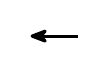
\begin{tikzpicture}
		\draw[->, thick, >={Stealth[round]}, line width=0.4mm] (0.3,0) -- (-0.3,0);
		\end{tikzpicture}};
		
}

\newcommand\ArrowNL[3]
{
	\node at (#1+1, #2+0.5, #3-0.5) 
	%	\node at (#1, #2, #3) 
	{
		
\begin{tikzpicture}
		\draw[->, thick, >={Stealth[round]}, line width=0.4mm] (0.16,0.16) -- (-0.16,-0.16);
		\end{tikzpicture}};
	
}

\newcommand\ArrowNR[3]
{
	\node at (#1+0.5, #2+1, #3-0.5) 
	%	\node at (#1, #2, #3) 
	{
		
\begin{tikzpicture}
		\draw[->, thick, >={Stealth[round]}, line width=0.4mm] (0.16,0.16) -- (-0.16,-0.16);
		\end{tikzpicture}};
	
}

\newcommand\ArrowNW[3]
{
	\node at (#1+0.5, #2+0.5, #3) 
%	\node at (#1, #2, #3) 
	{
		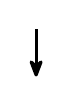
\begin{tikzpicture}
		\draw[->, thick, >={Stealth[round]}, line width=0.4mm] (0,0.3) -- (0,-0.3);
		\end{tikzpicture}};
	
}

\newcommand\ArrowSW[3]
{
	\node at (#1+0.5, #2+0.5, #3) 
%	\node at (#1, #2, #3) 
	{
		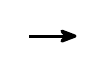
\begin{tikzpicture}
		\draw[<-, thick, >={Stealth[round]}, line width=0.4mm] (0.3,0) -- (-0.3,0);
		\end{tikzpicture}};
	
}

\newcommand\ArrowSE[3]
{
	\node at (#1+0.5, #2+0.5, #3) 
%	\node at (#1, #2, #3) 
	{
		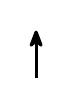
\begin{tikzpicture}
		\draw[<-, thick, >={Stealth[round]}, line width=0.4mm] (0,0.3) -- (0,-0.3);
		\end{tikzpicture}};
	
}

% Definition of \planepartition
% To draw the following plane partition, just write \planepartition{ {a, b, c}, {d,e} }.
%  a b c
%  d e
\newcommand\planepartition[1]{
	\setcounter{x}{-1}
	\foreach \a in {#1} {
		\addtocounter{x}{1}
		\setcounter{y}{-1}
		\foreach \b in \a {
			\addtocounter{y}{1}
			\setcounter{z}{-1}
			\foreach \c in {0,...,\b} {
				\addtocounter{z}{1}
				\ifthenelse{\c=0}{\setcounter{z}{-1},\addtocounter{y}{0}}{
					\cube{\value{x}}{\value{y}}{\value{z}}}
			}
		}
	}
}


%%\begin{tikzpicture}[x=(220:1cm), y=(-40:1cm), z=(90:0.707cm)]
	%\planepartition{{0,0,1},{1,1,1},{1,0,0},{1,0,1}};
\foreach \m [count=\y] in {{1,1,1,1},{1,1,1},{1,1,1,1},{1,1,1}}{
	\foreach \n [count=\x] in \m {
		\ifnum \n>0
		\foreach \z in {1,...,\n}{
			\draw [fill=blue!30] (\x+1,\y,\z) -- (\x+1,\y+1,\z) -- (\x+1, \y+1, \z-1) -- (\x+1, \y, \z-1) -- cycle;
			\draw [fill=blue!40] (\x,\y+1,\z) -- (\x+1,\y+1,\z) -- (\x+1, \y+1, \z-1) -- (\x, \y+1, \z-1) -- cycle;
			\draw [fill=blue!10] (\x,\y,\z)   -- (\x+1,\y,\z)   -- (\x+1, \y+1, \z)   -- (\x, \y+1, \z) -- cycle;  
		}
	
		\fi
	}
}   

\foreach \m [count=\y] in {{0,0,0,1}, {0,0,0}} {
	\foreach \n [count=\x] in \m {
		\ifnum \n>0
		\foreach \z in {1,...,\n}{
			\draw [fill=green!30] (\x+1,\y,\z) -- (\x+1,\y+1,\z) -- (\x+1, \y+1, \z-1) -- (\x+1, \y, \z-1) -- cycle;
			\draw [fill=green!40] (\x,\y+1,\z) -- (\x+1,\y+1,\z) -- (\x+1, \y+1, \z-1) -- (\x, \y+1, \z-1) -- cycle;
			\draw [fill=green!10] (\x,\y,\z)   -- (\x+1,\y,\z)   -- (\x+1, \y+1, \z)   -- (\x, \y+1, \z) -- cycle;  
		}
		
		\fi
	}
}   

\ArrowNW{1}	{3}	{1};

\foreach \m [count=\y] in {{0,0,0,0},{0,0,0},{0,0,0,0},{2,0,0}}{
	\foreach \n [count=\x] in \m {
		\ifnum \n>0
		\foreach \z in {1,...,\n}{
			\draw [fill=orange!30] (\x+1,\y,\z) -- (\x+1,\y+1,\z) -- (\x+1, \y+1, \z-1) -- (\x+1, \y, \z-1) -- cycle;
			\draw [fill=orange!40] (\x,\y+1,\z) -- (\x+1,\y+1,\z) -- (\x+1, \y+1, \z-1) -- (\x, \y+1, \z-1) -- cycle;
			\draw [fill=orange!10] (\x,\y,\z)   -- (\x+1,\y,\z)   -- (\x+1, \y+1, \z)   -- (\x, \y+1, \z) -- cycle;  
		}
		
		\fi
	}
}  

\foreach \m [count=\y] in {{0},{0},{0},{0,1,1}}{
	\foreach \n [count=\x] in \m {
		\ifnum \n>0
		\foreach \z in {1,...,\n}{
			\draw [fill=blue!30] (\x+1,\y,\z) -- (\x+1,\y+1,\z) -- (\x+1, \y+1, \z-1) -- (\x+1, \y, \z-1) -- cycle;
			\draw [fill=blue!40] (\x,\y+1,\z) -- (\x+1,\y+1,\z) -- (\x+1, \y+1, \z-1) -- (\x, \y+1, \z-1) -- cycle;
			\draw [fill=blue!10] (\x,\y,\z)   -- (\x+1,\y,\z)   -- (\x+1, \y+1, \z)   -- (\x, \y+1, \z) -- cycle;  
		}
		
		\fi
	}
} 

\foreach \m [count=\y] in {{0},{0},{0},{1,0,0}}{
	\foreach \n [count=\x] in \m {
		\ifnum \n>0
		\foreach \z in {1,...,\n}{
		%	\draw [fill=blue!30] (\x+1,\y,\z) -- (\x+1,\y+1,\z) -- (\x+1, \y+1, \z-1) -- (\x+1, \y, \z-1) -- cycle;
			\draw [fill=blue!40] (\x,\y+1,\z) -- (\x+1,\y+1,\z) -- (\x+1, \y+1, \z-1) -- (\x, \y+1, \z-1) -- cycle;
		%	\draw [fill=blue!10] (\x,\y,\z)   -- (\x+1,\y,\z)   -- (\x+1, \y+1, \z)   -- (\x, \y+1, \z) -- cycle;  
		}
		
		\fi
	}
} 
		"x" "y" "z"

\ArrowNR{4} {1}	{1};
\ArrowNL{4} {1}	{1};

\ArrowNR{4} {3}	{1};
\ArrowNL{4} {3}	{1};

\ArrowNR{3} {4}	{1};
\ArrowNL{3} {4}	{1};

\ArrowNR{1} {4}	{1};
\ArrowNR{2} {4}	{1};

\ArrowNL{3} {2}	{1};

\ArrowSW{1}	{1}	{1};
\ArrowSW{2}	{1}	{1};
\ArrowSW{3}	{1}	{1};
\ArrowSW{4}	{1}	{1};


\ArrowNW{1}	{2}	{1};
\ArrowSW{2}	{2}	{1};
\ArrowNW{3}	{2}	{1};

\ArrowNW{2}	{3}	{1};
\ArrowNE{3}	{3}	{1};
\ArrowNE{4}	{3}	{1};

%\ArrowNW{1}	{4}	{1};
\ArrowSW{2}	{4}	{1};
\ArrowNW{3}	{4}	{1};

%
%	\caption{large structure}
%
%	\label{fig:cover2}
%\end{figure}
%
%\begin{figure}[htb]
%
%  \centering
%  \includegraphics[width=3.4in]{Figures/cover.png}
%
%  \caption{M-Bocks modular robots with connections illuminated with onboard LEDs}
%
%  \label{fig:cover}
%\end{figure}



%%%%%%%%%%%%%%%%%%%%%%%%%%%%%%%%%%%%%%%%%%%%%%%%%%%%%%%%%%%%%%%%%%%%%%%%%%%%%%%%%%%%%%%%%%%%%%%%%%%%%%%%%%%%%%%%%%%%%%%%%%%%%%%%%%%%%%%%%%%%%%%
%%%%%%%%%%%%%%%%%%%%%%%%%%%%%%%%%%%%%%%%%%%%%%%%%%%%%%%%%%%%%%%%%%%%%%%%%%%%%%%%%%%%%%%%%%%%%%%%%%%%%%%%%%%%%%%%%%%%%%%%%%%%%%%%%%%%%%%%%%%%%%%
\section{Related Work}
\label{sec:RelatedWork}

\begin{table*}[t]
	\centering
	\caption{Comparison of attributes for several tagging technologies utilized by MSRR systems in order to determine the configuration of assemblies of modules.}
	\newcommand{\wdd}{2.0cm}
	\begin{tabular}{ p{2.4 cm} p{\wdd}  p{\wdd} p{\wdd} p{\wdd} p{\wdd} p{\wdd} p{\wdd}  }
		\hline
		\addlinespace[1ex]
		%1 - EMPTY
													& RFID / NFC		& Optical				& Electrical 		& QR Codes 			& Inductive				& \bf{\tagNamePlural} 		\\ %8
		\hline
		
		\addlinespace[0.5ex]	\textit{Information Storage or transfe medium}	& Radio waves		& IR or visible light	& Direct wired communication	& 2D optical grid	& Inductive				& Permanent Magnet Field	\\
		
		\addlinespace[0.5ex]	\textit{Tag Cost}		& Cheap				& Moderate				& Cheap				& Cheap	 			& Moderate				& Inexpensive 				\\
		
		\addlinespace[0.5ex]	\textit{Reader Cost}	& Expensive			& Moderate				& Moderate			& Expensive 	 	& Moderate				& Moderate 					\\
		
	%	\addlinespace[0.5ex] 	\textit{Size} 			& significant 		& minimal 				& minimal	  		& small      		& varies				& Small		  				\\
		
		\addlinespace[0.5ex]	\textit{Passive} 		& yes				& no					& possible	 		& yes				& no					& Yes		  				\\
		
		\addlinespace[0.5ex]	\textit{Communication} 	& possible			& yes					& yes	 			& no				& yes					& not yet		  			\\
		
		\addlinespace[0.5ex] 	\textit{Orientation} 	& needs 4 tags 		& possible 				& possible	 		& yes				& needs 4+ points		& Yes						\\
		
		\addlinespace[1ex] 	\textit{MSRR Systems}
		& ~\cite{StigmergyWerfel2006}	%RFID	
		& CK-Bot~\cite{park2008automatic}					%OPTICAL
		& ~\cite{Soldercubes2016}, ~\cite{ubot-Zhu-2014}	%Electrical
		& ~\cite{lin2017vision}								%QR Codes 
		& ~\cite{TosunDaveyLiuYim-IROS2016}					%Inductive
		& 3D M-Blocks~\cite{Romanishin20153d}	\\ 			%M-Tags
		
		\addlinespace[1ex] 	\textit{Range}			& 0-10$m$			& variable				& 0 mm				& ~10mm +			& ~10mm +			& 0-1$mm$	\\
	\end{tabular}
	\label{tab:tagTech}
\end{table*}

%%%%%%%%%%%%%%%%%%%%%%%%%%%%%%%%%%%%%%%%%%%%%%%%%%%%%%%%%%%%%%%%%%%%%%%%%%%%%%%%%%%%%%%%%%%%%%%%%%%%%%%%%%%%%%%%%%%%%%%%%%%%%%%%%%%%%%%%%%%%%%%
%%%%%%%%%%%%%%%%%%%%%%%%%%%%%%%%%%%%%%%%%%%%%%%%%%%%%%%%%%%%%%%%%%%%%%%%%%%%%%%%%%%%%%%%%%%%%%%%%%%%%%%%%%%%%%%%%%%%%%%%%%%%%%%%%%%%%%%%%%%%%%%

Many papers provide a comprehensive overviews of the MSRR field including the seminal article published in 2007~\cite{Yim-RAM07} in addition to several ore recent updates, including~\cite{chennareddy2017modular} which focuses on the hardware systems, and ~\cite{abukhalil2013survey} which focuses on algorithmic developments. This section of the paper will attempt to investigate two different topics in the related work in a more focused manner, Subsection~\ref{ssec:RWconfiguration} will look at the challenge of configuration discovery in modular robotics systems, Finally Subsection~\ref{ssec:RW-Algorithmic} touches on some of the work implementing similar behaviors to those described in this work.

%%%%%%%%%%%%%%%%%%%%%%%%%%%%%%%%%%%%%%%%%%%%%%%%%%%%%%%%%%%%%%%%%%%%%%%%%%%%%%%%%%%%%%%%%%%%%%%%%%%%%%%%%%%%%%%%%%%%%%%%%%%%%%%%%%%%%%%%%%%%%%%
%%%%%%%%%%%%%%%%%%%%%%%%%%%%%%%%%%%%%%%%%%%%%%%%%%%%%%%%%%%%%%%%%%%%%%%%%%%%%%%%%%%%%%%%%%%%%%%%%%%%%%%%%%%%%%%%%%%%%%%%%%%%%%%%%%%%%%%%%%%%%%%
\subsection{Configuration Discovery in MSRR Systems}
\label{ssec:RWconfiguration}
%%%%%%%%%%%%%%%%%%%%%%%%%%%%%%%%%%%%%%%%%%%%%%%%%%%%%%%%%%%%%%%%%%%%%%%%%%%%%%%%%%%%%%%%%%%%%%%%%%%%%%%%%%%%%%%%%%%%%%%%%%%%%%%%%%%%%%%%%%%%%%%
%%%%%%%%%%%%%%%%%%%%%%%%%%%%%%%%%%%%%%%%%%%%%%%%%%%%%%%%%%%%%%%%%%%%%%%%%%%%%%%%%%%%%%%%%%%%%%%%%%%%%%%%%%%%%%%%%%%%%%%%%%%%%%%%%%%%%%%%%%%%%%%
Connectors are one of the most significant design challenges in creating practical MSRR systems. Aside from their fundamental requirement of providing robust mechanical links, these connectors have been used in the literature to enable inter-module communication \cite{liedke2013collective}, \cite{TosunDaveyLiuYim-IROS2016}, deliver power to modules \cite{OptimalPowerSharing2016}, and determine the presence and relative orientation of adjacent units. While all of these improvements to inter-module connections are extensively explored by other researchers, solutions for gathering information about units are limited, and generally require both units to be active.  This paper focuses on this feature of connectors, looks at an overview of how location and identity information is encoded in connectors, and proposes a new method which the authors believe compares favorably with the existing state of the art.
	
Work has been done attempting to discover the configuration of groups of modules, including in ~\cite{park2008automatic}
The ability for a modular system to discover the specific configuration of modules at any and all times is one of the most essential tasks for any modular robotic system. However, many of the modular robotic systems proposed to date have either built very limited and error prone methods for solving this problem, or have omitted implementation of such a system entirely. Any \textbf{connection} between modules in a modular system involves a minimum of three unique parameters 1) Some form of Identity or \textbf{ID} of the two modules in question, 2) the connector, or \textbf{face number} for each of the modules, and 3) the \textbf{orientation} of the connection, which in a cubic lattice is one of four possible 90 degree values.

Many of the existing systems have faces which are able to pass information locally. This communication be used to discover the face number and the module ID's, but we are not aware of any of these systems which are able to systematically discover the orientation of the connection. Some systems combine connectivity information determined from face-to-face connections with gravity measurements from accelerometers to construct data structures which represent both module adjacency and relative orientations \cite{Soldercubes2016}; however, because the gravity field is locally uniform, there are some module arrangements where accelerometer measurements cannot completely determine relative orientation.

Two of the most problematic aspects of current systems we have identified are the need for both modules involved to be actively. A lack of robust connector orientation information, and the large expense and complexity associated with implementing many multiples of these systems.


%%%%%%%%%%%%%%%%%%%%%%%%%%%%%%%%%%%%%%%%%%%%%%%%%%%%%%%%%%%%%%%%%%%%%%%%%%%%%%%%%%%%%%%%%%%%%%%%%%%%%%%%%%%%%%%%%%%%%%%%%%%%%%%%%%%%%%%%%%%%%%%
%%%%%%%%%%%%%%%%%%%%%%%%%%%%%%%%%%%%%%%%%%%%%%%%%%%%%%%%%%%%%%%%%%%%%%%%%%%%%%%%%%%%%%%%%%%%%%%%%%%%%%%%%%%%%%%%%%%%%%%%%%%%%%%%%%%%%%%%%%%%%%%
\subsection{Relevant MSRR algorithmic work}
\label{ssec:RW-Algorithmic}
%%%%%%%%%%%%%%%%%%%%%%%%%%%%%%%%%%%%%%%%%%%%%%%%%%%%%%%%%%%%%%%%%%%%%%%%%%%%%%%%%%%%%%%%%%%%%%%%%%%%%%%%%%%%%%%%%%%%%%%%%%%%%%%%%%%%%%%%%%%%%%%
%%%%%%%%%%%%%%%%%%%%%%%%%%%%%%%%%%%%%%%%%%%%%%%%%%%%%%%%%%%%%%%%%%%%%%%%%%%%%%%%%%%%%%%%%%%%%%%%%%%%%%%%%%%%%%%%%%%%%%%%%%%%%%%%%%%%%%%%%%%%%%%
While there are many simulated algorithms to accomplish similar behaviors, much of these works and assume and abstract away various challenges that real-world modules would face. There are many works introducing various algorithms and control strategies, and we are not claiming that those presented in "behaviors" are in any way unique. This work from 2014~\cite{abukhalil2013survey}, provides an overview of some of the existing academic work involving decentralized control strategies. Light tracking behaviors can be traced to the canonical Braitenberg vehicles~\cite{braitenberg1986vehicles}, in addition to several papers detailing control strategies for MSRR~\cite{claici2017distributed}.


%	For modular robots, knowing which neighbors each module is connected to and the relative angle of that connection is indispensable for MSRR systems. While systems have left this problem un-addressed, most MSRR systems have some method to determine the configuration. Some connections also implement inter-module communication between modules using the same hardware used for configuration detection. Other systems use passive methods like RFID tags, e.g.\cite{Werfel-PhDThesis06} to sense module adjacency. 
%inclusion of ``passive'' modules in the robot as described by \cite{roombots-Bonardi-2013}. 
% Other systems use RFID tags \cite{Werfel-PhDThesis06} to explicitly sense module adjacency.
% implicitly sense adjacent neighbors \cite{liedke2013collective} \cite{Gilpin-Thesis06} \cite{TosunDaveyLiuYim-IROS2016}. 
%%%%%%%%%%%%%%%%%%%%%%%%%%%%%%%%%%%%%%%%%%%%%%%%%%%%%%%%%%%%%%%%%%%%%%%%%%%%%%%%%%%%%%%%%%%%%%%%%%%%%%%%%%%%%%%%%%%%%%%%%%%%%%%%%%%%%%%%%%%%%%%%
%%%%%%%%%%%%%%%%%%%%%%%%%%%%%%%%%%%%%%%%%%%%%%%%%%%%%%%%%%%%%%%%%%%%%%%%%%%%%%%%%%%%%%%%%%%%%%%%%%%%%%%%%%%%%%%%%%%%%%%%%%%%%%%%%%%%%%%%%%%%%%%%
%\subsection{Location Tagging technology overview}
%\label{ssec:RWtaggingTech}
%%%%%%%%%%%%%%%%%%%%%%%%%%%%%%%%%%%%%%%%%%%%%%%%%%%%%%%%%%%%%%%%%%%%%%%%%%%%%%%%%%%%%%%%%%%%%%%%%%%%%%%%%%%%%%%%%%%%%%%%%%%%%%%%%%%%%%%%%%%%%%%%
%%%%%%%%%%%%%%%%%%%%%%%%%%%%%%%%%%%%%%%%%%%%%%%%%%%%%%%%%%%%%%%%%%%%%%%%%%%%%%%%%%%%%%%%%%%%%%%%%%%%%%%%%%%%%%%%%%%%%%%%%%%%%%%%%%%%%%%%%%%%%%%%
%
%There are several different types of passive tagging technologies designed allow a reader to extract unique identification numbers from tags. These include RFID, NFC, QR-Codes, April Tags~\cite{wang2016iros}. This section will provide a brief discussion of the characteristics of each of these technologies, and their suitability to working in the context of cm module scale MSRR systems. Table~\ref{tab:tagTech} provides an over and a (subjective) comparison between several of these technologies, and a listing of several example multi-robot systems which utilize this approach for broadly similar configuration detection roles.

%%%%%%%%%%%%%%%%%%%%%%%%%%%%%%%%%%%%%%%%%%%%%%%%%%%%%%%%%%%%%%%%%%%%%%%%%%%%%%%%%%%%%%%%%%%%%%%%%%%%%%%%%%%%%%%%%%%%%%%%%%%%%%%%%%%%%%%%%%%%%%%
%%%%%%%%%%%%%%%%%%%%%%%%%%%%%%%%%%%%%%%%%%%%%%%%%%%%%%%%%%%%%%%%%%%%%%%%%%%%%%%%%%%%%%%%%%%%%%%%%%%%%%%%%%%%%%%%%%%%%%%%%%%%%%%%%%%%%%%%%%%%%%%
\section{Hardware}
\label{sec:Hardware}
%%%%%%%%%%%%%%%%%%%%%%%%%%%%%%%%%%%%%%%%%%%%%%%%%%%%%%%%%%%%%%%%%%%%%%%%%%%%%%%%%%%%%%%%%%%%%%%%%%%%%%%%%%%%%%%%%%%%%%%%%%%%%%%%%%%%%%%%%%%%%%%
%%%%%%%%%%%%%%%%%%%%%%%%%%%%%%%%%%%%%%%%%%%%%%%%%%%%%%%%%%%%%%%%%%%%%%%%%%%%%%%%%%%%%%%%%%%%%%%%%%%%%%%%%%%%%%%%%%%%%%%%%%%%%%%%%%%%%%%%%%%%%%%

This section introduces the new magnetic fiducial tags (MFTags) which are implemented on the 3D M-Block Modules, originally presented in~\cite{RomanishinRus-IROS13} and extended to 3D in~\cite{Romanishin20153d}. Basic information regarding 3D M-Blocks is presented in Table~\ref{tab:hardwareOverviewTable}. These modules can pivot on a cubic lattice using pulses of angular momentum from an internal reaction wheel according to the pivoting cube model, but were not able to effectively determine their neighbor connectivity or communicate through their faces. 
%%%%%%%%%%%%%%%%%%%%%%%%%%%%%%%%%%%%%%%%%%%%%%%%%%%%%%%%%%%%%%%%%%%%%%%%%%%%%%%%%%%%%%%%%%%%%%%%%%%%%%%%%%%%%%%%%%%%%%%%%%%%%%%%%%%%%%%%%%%%%%%
%%%%%%%%%%%%%%%%%%%%%%%%%%%%%%%%%%%%%%%%%%%%%%%%%%%%%%%%%%%%%%%%%%%%%%%%%%%%%%%%%%%%%%%%%%%%%%%%%%%%%%%%%%%%%%%%%%%%%%%%%%%%%%%%%%%%%%%%%%%%%%%
\begin{table}[h]
	\caption{Basic info of the m-Blocks modular robots}
	
	\begin{tabular}{ p{3.4cm}  p{1.9cm} }
		\hline
		Actuation Directions & 6 \\
		Mass  & 163\,g \\
		Characterist Dimension & 50\,mm \\dra
		Total Parts  & 216 \\
		Actuated Moving Parts  & 10 \\
	%	Est. Cost & \$230 \\
	\end{tabular}
	
	\label{tab:hardwareOverviewTable}
\end{table}
%%%%%%%%%%%%%%%%%%%%%%%%%%%%%%%%%%%%%%%%%%%%%%%%%%%%%%%%%%%%%%%%%%%%%%%%%%%%%%%%%%%%%%%%%%%%%%%%%%%%%%%%%%%%%%%%%%%%%%%%%%%%%%%%%%%%%%%%%%%%%%%
%%%%%%%%%%%%%%%%%%%%%%%%%%%%%%%%%%%%%%%%%%%%%%%%%%%%%%%%%%%%%%%%%%%%%%%%%%%%%%%%%%%%%%%%%%%%%%%%%%%%%%%%%%%%%%%%%%%%%%%%%%%%%%%%%%%%%%%%%%%%%%%

In order to include this functionality this section introduces the \TagNamePlural, which is a new fiducial tag system which allows modules to detect information about their neighbors. The important design criteria taken into consideration while designing \TagNamePlural include the following:
\begin{itemize}
	\item Passive - information can be read even when the module is inactive.
	\item Inexpensive - necessary for scaling systems of beyond 1000 of modules.
	\item Unique identities - needs to provide accurate location for large systems.
	\item Orientation - the tag needs to reliably determine the 90-degree angle relative to the reader.
\end{itemize} 

Our new method for estimating the position of adjacent modules addresses both of these issues, and is illustrated with in Figure~\ref{fig:tagDiagram8}. \TagNamePlural are essentially arrangements of magnets mounted on the faces of modules.  The orientation of magnets which comprise \tagNamePlural can be measured by simple absolute magnetic encoder ICs, thereby reading information encoded in the orientation of the magnets.

%%%%%%%%%%%%%%%%%%%%%%%%%%%%%%%%%%%%%%%%%%%%%%%%%%%%%%%%%%%%%%%%%%%%%%%%%%%%%%%%%%%%%%%%%%%%%%%%%%%%%%%%%%%%%%%%%%%%%%%%%%%%%%%%%%%%%%%%%%%%%%%
%%%%%%%%%%%%%%%%%%%%%%%%%%%%%%%%%%%%%%%%%%%%%%%%%%%%%%%%%%%%%%%%%%%%%%%%%%%%%%%%%%%%%%%%%%%%%%%%%%%%%%%%%%%%%%%%%%%%%%%%%%%%%%%%%%%%%%%%%%%%%%%
\begin{table}[b]
	\caption{Information content in the \TagNamePlural encoding specification. The current system is limited due to practical considerations of the physical dimensions of the  PCBa's in the 3D M-Blocks, but will hopefully be extended into the future extension soon.}
	
	\begin{tabular}{ p{2cm}  p{1.5cm}  p{1.5cm}  p{1.5cm}}
		\hline
								& \textit{Current System} & Future Extension & Advanced Extended \\
		\hline
				\addlinespace[1ex]
		Magnets  				& 4 			 &	4				&	4	\\
		Digits 					& 30 			 &	24				&	48	\\
		No. Of Sensors 			& 2 			 &	4				&	4	\\
		\textit{Unique Tags} 	& \textbf{900} 	 & 331776			& 	~5,000,000\\
		
	\end{tabular}
	
	\label{tab:hardwareOverview}
\end{table}
%%%%%%%%%%%%%%%%%%%%%%%%%%%%%%%%%%%%%%%%%%%%%%%%%%%%%%%%%%%%%%%%%%%%%%%%%%%%%%%%%%%%%%%%%%%%%%%%%%%%%%%%%%%%%%%%%%%%%%%%%%%%%%%%%%%%%%%%%%%%%%%
%%%%%%%%%%%%%%%%%%%%%%%%%%%%%%%%%%%%%%%%%%%%%%%%%%%%%%%%%%%%%%%%%%%%%%%%%%%%%%%%%%%%%%%%%%%%%%%%%%%%%%%%%%%%%%%%%%%%%%%%%%%%%%%%%%%%%%%%%%%%%%%

The approach that \tagNamePlural~take towards this problem is a passive magnetic connector that uses a combination of dipole angles to communicate identity and relative rotational position. In this implementation, each face of each cube is encoded with a different combination of magnetic angles than every other face of every other cube. Magnetic rotary position sensors read these dipole angle combinations to determine which face is directly adjacent, and they identify the rotational angle of the face as well. All of this occurs using an un-powered array of magnets that provide static EM fields, readable at a hyperlocal distance.

The underlying hypothesis is that low cost and lack of RF transmission make magnets an attractive choice for a technology that may have to be implemented hundreds of times in a set of reconfigurable modules. The ability to use several such sensors at close proximity allows several to be used on each connecting face, providing enough data to read configuration as well as identity. The \tagNamePlural were designed and tested with the M-Blocks modular robots as the test bed, although nothing precludes their use in other circumstances.

%%%%%%%%%%%%%%%%%%%%%%%%%%%%%%%%%%%%%%%%%%%%%%%%%%%%%%%%%%%%%%%%%%%%%%%%%%%%%%%%%%%%%%%%%%%%%%%%%%%%%%%%%%%%%%%%%%%%%%%%%%%%%%%%%%%%%%%%%%%%%%%
%%%%%%%%%%%%%%%%%%%%%%%%%%%%%%%%%%%%%%%%%%%%%%%%%%%%%%%%%%%%%%%%%%%%%%%%%%%%%%%%%%%%%%%%%%%%%%%%%%%%%%%%%%%%%%%%%%%%%%%%%%%%%%%%%%%%%%%%%%%%%%%
%%%%%%%%%%%%%%%%%%%%%%%%%%%%%%%%%%%%%%%%%%%%%%%%%%%%%%%%%%%%%%%%%%%%%%%%%%%%%%%%%%%%%%%%%%%%%%%%%%%%%%%%%%%%%%%%%%%%%%%%%%%%%%%%%%%%%%%%%%%%%%%
%%%%%%%%%%%%%%%%%%%%%%%%%%%%%%%%%%%%%%%%%%%%%%%%%%%%%%%%%%%%%%%%%%%%%%%%%%%%%%%%%%%%%%%%%%%%%%%%%%%%%%%%%%%%%%%%%%%%%%%%%%%%%%%%%%%%%%%%%%%%%%%
\begin{figure*}[th]
	
	\newsavebox{\faceDiagram}
	\sbox{\faceDiagram}	{
		\newcommand{\statcirc}[4]{
	\fill[red,shift={(#1 cm,#2 cm)}, rotate=#3] (0,0) circle (#4); 
	\fill[blue,shift={(#1 cm,#2 cm)},rotate=#3] (0,0) -- (180:#4) arc (180:0:#4) -- cycle;
	%	\draw[->,black,shift={(#1 cm,#2 cm)},rotate=#3] (#4, 0)
}

\newcommand{\drawArrow}[3]{
	\draw[->,>={Stealth[round]}, line width=0.75mm, black ,shift={(#1 cm,#2 cm)}, rotate=#3] (0,-0.5) -- (0,0.5); 
}

\newcommand{\drawchip}[3]{
	\tikzmath
	{
		\chipW = 0.35;
		\chipH = 0.4;
	}
	\fill[darkgray, shift= {(#1 cm, #2 cm)}, rotate = #3, rounded corners] (-\chipH,-\chipW) rectangle (\chipH,\chipW);
	\fill[orange,shift= {(#1 cm, #2 cm)}, rotate = #3 ] (-0.25,0.2) circle (0.1);
}
\begin{tikzpicture}

	\tikzmath{
		\offsetAxis = 0.5;
		\offsetCent = 2.9;
		\diameter = 0.32;
	}
	\draw node (A) at (-0.5, 2.2) {};
	\draw node (B) at (0, 2.2) {};
	\drawchip{\offsetAxis}{\offsetCent}{0};
	\drawchip{-\offsetAxis}{-\offsetCent}{180};
	\statcirc{-\offsetAxis}{\offsetCent}{30}{\diameter};
	\drawArrow{-\offsetAxis}{\offsetCent}{30}
	\statcirc{\offsetCent}{\offsetAxis}{210}{\diameter};
	\statcirc{\offsetAxis}{-\offsetCent}{190}{\diameter};
	\statcirc{-\offsetCent}{-\offsetAxis}{45}{\diameter};
	\draw[gray, dashed] (-\offsetAxis,{\offsetCent + 1}) -- 
	(-\offsetAxis,{\offsetCent - 1});
	\draw[black,dotted] (0,0) circle (2.95);
	
	% 4 Cross Lines X
	\draw[black,dashed] (0,0) -- (4,0);
	\draw[black,dashed] (0,0) -- (-4,0);
	\draw[black,dashed] (0,0) -- (0,4);
	\draw[black,dashed] (0,0) -- (0,-4);
	
	% Dimensioned Variables
	\dimline[line style = {line width = 0.8, arrows = dimline reverse-dimline reverse}] {(A)}{(B)}{x};
	\dimline[line style = {line width = 0.8}] {(0,0)} {++(150:2.95)}{R};
%	\dimline {(1,0)}{(-1,0)}{x};
\end{tikzpicture}
	}
	
	\newsavebox{\magnetDigitization}
	\sbox{\magnetDigitization}	{
		
\newcommand{\statcirc}[4]{
	\fill[red,shift={(#1 cm,#2 cm)}, rotate=#3] (0,0) circle (#4); 
	\fill[blue,shift={(#1 cm,#2 cm)},rotate=#3] (0,0) -- (180:#4) arc (180:0:#4) -- cycle;
	%	\draw[->,black,shift={(#1 cm,#2 cm)},rotate=#3] (#4, 0)
}

\newcommand{\drawArrow}[3]{
	\draw[->,>={Stealth[round]}, line width=0.75mm, black ,shift={(#1 cm,#2 cm)}, rotate=#3] (0,-1) -- (0,1); 
}

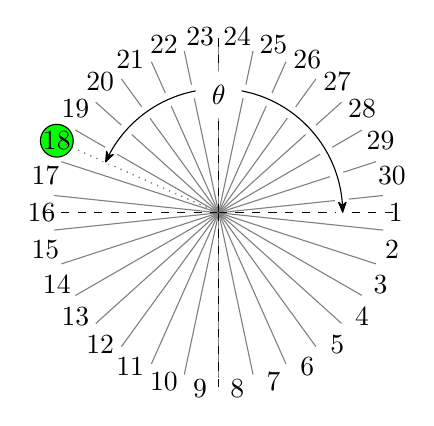
\begin{tikzpicture}[scale = 0.75]
\tikzmath{
	\offsetAxis = 0.5;
	\offsetCent = 2.9;
	\diameter = 0.75;
}

\foreach \i in {1,...,30}
{
	\draw[gray] (0,0) -- (\i * 12-6 : 2.8);
	\node[inner sep=0pt] at (-{\i * 12}+12: 3) {\i};
}
\node[circle,draw,inner sep=0pt, fill = green] at (-{18 * 12}+12: 3) {18};
\statcirc{0}{0}{-204-90}{\diameter};
\drawArrow{0}{0}{-204-90};
\draw[black,dashed] (0,0) -- (3,0);
\draw[black,dashed] (0,0) -- (-3,0);
\draw[black,dashed] (0,0) -- (0,3);
\draw[black,dashed] (0,0) -- (0,-3);
\draw[gray, dotted] (0,0) -- (-204: 3);
\draw[gray, dotted] (0,0) -- (-204: 3);
\draw [white, line width = 5pt] (2.1,0)  arc (0:360-204:2.1);
\draw [<->, >={Stealth[round]}] (2.1,0)  arc (0:360-204:2.1);
\node[circle,inner sep=3pt, fill = white]				at (90:2) {$\theta$};
\end{tikzpicture}
	}
	
	\newsavebox{\gridFigure}
	\sbox{\gridFigure}	{
		

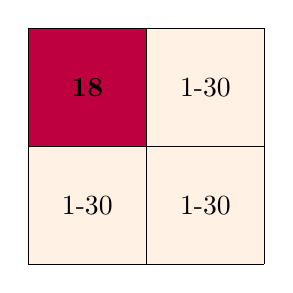
\begin{tikzpicture}[every node/.style={minimum size=1.5 cm-\pgflinewidth, outer sep=0pt}]
	\tikzmath{
		\boxSize = 1.5;
	}

    \draw[step= \boxSize cm,color=black] (0,0) grid (\boxSize*2,\boxSize*2);
	
    \node[fill=orange!10] at (\boxSize*1.5,\boxSize*1.5 ) {1-30};
    \node[fill=orange!10] at (\boxSize*0.5,\boxSize*0.5) {1-30};
    \node[fill=purple] at (\boxSize*0.5,\boxSize*1.5) {\textbf{18}};
    \node[fill=orange!10] at (\boxSize*1.5,\boxSize*0.5) {1-30};
   % \node[fill=yellow] at (+0.75,+0.75) {};
\end{tikzpicture}
	}
	%\begin{tikzpicture}[minimum width = 14 cm, minimum height = 6 cm]
	%\draw (0,0) -- (14,6);
	
	\begin{tikzpicture}[]
	%complexnode/.pic={\usebox{\mybox}}]
	
	\newcommand\xa{2};
	\newcommand\xb{2};
	\newcommand\ya{2};
	\newcommand\yb{2};
	
	\coordinate (smallNE) at (2,5);
	\coordinate (smallSE) at (2,5);
	\coordinate (smallSW) at (2,5);
	\coordinate (smallNW) at (2,5);
	
	\coordinate (bigNE) at (2,5);
	\coordinate (bigSE) at (2,5);
	\coordinate (bigSW) at (2,5);
	\coordinate (bigSE) at (2,5);
	
	\node[opacity = 0.95] at (3.15 cm, 2.85 cm) {\includegraphics[width = 5.9 cm]{figures/face.png}};
	\node at (3 cm, 3 cm) {\usebox{\faceDiagram}};
	\node at (10 cm, 3 cm) {\usebox{\magnetDigitization}};
	\node at (15.5 cm, 2cm) {\usebox{\gridFigure}};
	
	%\node[fill=orange] at (3,3) {\textbf{18}};
	
	\tikzmath{
		\smallBoxX = 0.5;
		\smallBoxY = 2.9;
	}

	% Small Box around Magnet
	%\node[draw, purple, dotted, minimum size = 1.25 cm, rounded corners, thick] at (3.65cm , 7cm) {};
	
	\path[draw, purple, dotted, minimum size = 1.25 cm, rounded corners, ultra thick]
	(3*0.7, 6.25*0.7) --
	++(1.25, 0) --
	++(0, 1.25) --
	++(-1.25, 0) --
	cycle {};
	
	\node (a) at (12.5, 3){};
	\node (b) at (14.75, 3.4){};
	
	\draw[>={Stealth[round]}, purple,dashed, ultra thick, bend right, rounded corners = 1 cm, ->] (a) -- (13.75,5) -- (b);
	
	\draw[purple,dashed, thin] (2.7cm, 4.35cm + 1.25cm) -- ++(358: 4.8cm);
	\draw[purple,dashed, thin] (2.7cm, 4.35cm ) -- ++(323: 5.9cm);
	
	% Large Purple box
	\node[draw, purple, dotted, minimum size = 5 cm, rounded corners,ultra thick] at (10cm , 3cm) {};
	
	\node[] at (10cm , 0.2cm) {Discretizing Angle};
	%\draw (1,1) pic {complexnode} (4,4);
	
	\end{tikzpicture}
	
	
	
	
%	\newsavebox{\faceDiagram}
%	\sbox{\faceDiagram}	{
%		\newcommand{\statcirc}[4]{
	\fill[red,shift={(#1 cm,#2 cm)}, rotate=#3] (0,0) circle (#4); 
	\fill[blue,shift={(#1 cm,#2 cm)},rotate=#3] (0,0) -- (180:#4) arc (180:0:#4) -- cycle;
	%	\draw[->,black,shift={(#1 cm,#2 cm)},rotate=#3] (#4, 0)
}

\newcommand{\drawArrow}[3]{
	\draw[->,>={Stealth[round]}, line width=0.75mm, black ,shift={(#1 cm,#2 cm)}, rotate=#3] (0,-0.5) -- (0,0.5); 
}

\newcommand{\drawchip}[3]{
	\tikzmath
	{
		\chipW = 0.35;
		\chipH = 0.4;
	}
	\fill[darkgray, shift= {(#1 cm, #2 cm)}, rotate = #3, rounded corners] (-\chipH,-\chipW) rectangle (\chipH,\chipW);
	\fill[orange,shift= {(#1 cm, #2 cm)}, rotate = #3 ] (-0.25,0.2) circle (0.1);
}
\begin{tikzpicture}

	\tikzmath{
		\offsetAxis = 0.5;
		\offsetCent = 2.9;
		\diameter = 0.32;
	}
	\draw node (A) at (-0.5, 2.2) {};
	\draw node (B) at (0, 2.2) {};
	\drawchip{\offsetAxis}{\offsetCent}{0};
	\drawchip{-\offsetAxis}{-\offsetCent}{180};
	\statcirc{-\offsetAxis}{\offsetCent}{30}{\diameter};
	\drawArrow{-\offsetAxis}{\offsetCent}{30}
	\statcirc{\offsetCent}{\offsetAxis}{210}{\diameter};
	\statcirc{\offsetAxis}{-\offsetCent}{190}{\diameter};
	\statcirc{-\offsetCent}{-\offsetAxis}{45}{\diameter};
	\draw[gray, dashed] (-\offsetAxis,{\offsetCent + 1}) -- 
	(-\offsetAxis,{\offsetCent - 1});
	\draw[black,dotted] (0,0) circle (2.95);
	
	% 4 Cross Lines X
	\draw[black,dashed] (0,0) -- (4,0);
	\draw[black,dashed] (0,0) -- (-4,0);
	\draw[black,dashed] (0,0) -- (0,4);
	\draw[black,dashed] (0,0) -- (0,-4);
	
	% Dimensioned Variables
	\dimline[line style = {line width = 0.8, arrows = dimline reverse-dimline reverse}] {(A)}{(B)}{x};
	\dimline[line style = {line width = 0.8}] {(0,0)} {++(150:2.95)}{R};
%	\dimline {(1,0)}{(-1,0)}{x};
\end{tikzpicture}
%	}
%	
%	\newsavebox{\magnetDigitization}
%	\sbox{\magnetDigitization}	{
%		
\newcommand{\statcirc}[4]{
	\fill[red,shift={(#1 cm,#2 cm)}, rotate=#3] (0,0) circle (#4); 
	\fill[blue,shift={(#1 cm,#2 cm)},rotate=#3] (0,0) -- (180:#4) arc (180:0:#4) -- cycle;
	%	\draw[->,black,shift={(#1 cm,#2 cm)},rotate=#3] (#4, 0)
}

\newcommand{\drawArrow}[3]{
	\draw[->,>={Stealth[round]}, line width=0.75mm, black ,shift={(#1 cm,#2 cm)}, rotate=#3] (0,-1) -- (0,1); 
}

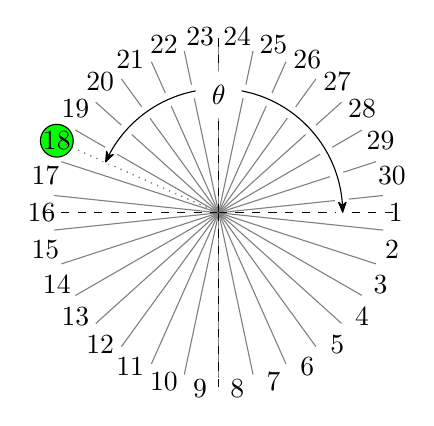
\begin{tikzpicture}[scale = 0.75]
\tikzmath{
	\offsetAxis = 0.5;
	\offsetCent = 2.9;
	\diameter = 0.75;
}

\foreach \i in {1,...,30}
{
	\draw[gray] (0,0) -- (\i * 12-6 : 2.8);
	\node[inner sep=0pt] at (-{\i * 12}+12: 3) {\i};
}
\node[circle,draw,inner sep=0pt, fill = green] at (-{18 * 12}+12: 3) {18};
\statcirc{0}{0}{-204-90}{\diameter};
\drawArrow{0}{0}{-204-90};
\draw[black,dashed] (0,0) -- (3,0);
\draw[black,dashed] (0,0) -- (-3,0);
\draw[black,dashed] (0,0) -- (0,3);
\draw[black,dashed] (0,0) -- (0,-3);
\draw[gray, dotted] (0,0) -- (-204: 3);
\draw[gray, dotted] (0,0) -- (-204: 3);
\draw [white, line width = 5pt] (2.1,0)  arc (0:360-204:2.1);
\draw [<->, >={Stealth[round]}] (2.1,0)  arc (0:360-204:2.1);
\node[circle,inner sep=3pt, fill = white]				at (90:2) {$\theta$};
\end{tikzpicture}
%	}
%	
%	\newsavebox{\gridFigure}
%	\sbox{\gridFigure}	{
%		

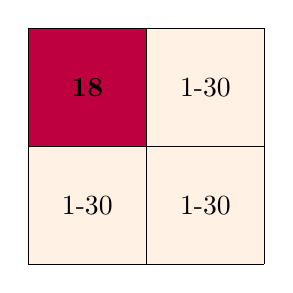
\begin{tikzpicture}[every node/.style={minimum size=1.5 cm-\pgflinewidth, outer sep=0pt}]
	\tikzmath{
		\boxSize = 1.5;
	}

    \draw[step= \boxSize cm,color=black] (0,0) grid (\boxSize*2,\boxSize*2);
	
    \node[fill=orange!10] at (\boxSize*1.5,\boxSize*1.5 ) {1-30};
    \node[fill=orange!10] at (\boxSize*0.5,\boxSize*0.5) {1-30};
    \node[fill=purple] at (\boxSize*0.5,\boxSize*1.5) {\textbf{18}};
    \node[fill=orange!10] at (\boxSize*1.5,\boxSize*0.5) {1-30};
   % \node[fill=yellow] at (+0.75,+0.75) {};
\end{tikzpicture}
%	}
%	%\begin{tikzpicture}[minimum width = 14 cm, minimum height = 6 cm]
%	%\draw (0,0) -- (14,6);
%	
%	\begin{tikzpicture}[]
%	%complexnode/.pic={\usebox{\mybox}}]
%	
%	\newcommand\xa{2};
%	\newcommand\xb{2};
%	\newcommand\ya{2};
%	\newcommand\yb{2};
%	
%	\coordinate (smallNE) at (2,5);
%	\coordinate (smallSE) at (2,5);
%	\coordinate (smallSW) at (2,5);
%	\coordinate (smallNW) at (2,5);
%	
%	\coordinate (bigNE) at (2,5);
%	\coordinate (bigSE) at (2,5);
%	\coordinate (bigSW) at (2,5);
%	\coordinate (bigSE) at (2,5);
%	
%	\node[opacity = 0.95] at (4.25 cm, 4 cm) {\includegraphics[width = 8 cm]{figures/face.png}};
%	\node at (4 cm, 4 cm) {\usebox{\faceDiagram}};
%	\node at (11 cm, 6 cm) {\usebox{\magnetDigitization}};
%	\node at (15 cm, 2cm) {\usebox{\gridFigure}};
%	
%	%\node[fill=orange] at (3,3) {\textbf{18}};
%	
%	\tikzmath{
%		\smallBoxX = 0.5;
%		\smallBoxY = 2.9;
%	}
%	
%	% Small Box around Magnet
%	%\node[draw, purple, dotted, minimum size = 1.25 cm, rounded corners, thick] at (3.65cm , 7cm) {};
%	
%	\path[draw, purple, dotted, minimum size = 1.25 cm, rounded corners, ultra thick]
%	(3, 6.25) --
%	++(1.25, 0) --
%	++(0, 1.25) --
%	++(-1.25, 0) --
%	cycle {};
%	
%	\node (a) at (13.5, 6){};
%	\node (b) at (15.75, 3.5){};
%	\draw[>={Stealth[round]}, purple,dashed, ultra thick, bend right, rounded corners = 1 cm, ->] (a) -- (15.75,6) -- (b);
%	\draw[purple,dashed, thin] (3.5cm, 6.25cm + 1.25cm) -- ++(10: 5cm);
%	\draw[purple,dashed, thin] (3.5cm, 6.25cm ) -- ++(332: 5.45cm);
%	
%	% Large Purple box
%	\node[draw, purple, dotted, minimum size = 4.8 cm, rounded corners,ultra thick] at (11cm , 6cm) {};
%	
%	%\draw (1,1) pic {complexnode} (4,4);
%	
%	\end{tikzpicture}
	
	\caption{Figure illustrating the \TagNamePlural. A tag consists of four permanent magnets placed according to two dimensions, (R) is the circle diameter, and x is the offset from the y axis. The right half of this figure shows a photo of one of the m-blocks superimposed with the magnets. The absolute angle of the magnet, relative to a line extending from the center of the face, is then digitized by an absolute magnetic encoder (black rectangle with orange dot) placed $x$ units to the right. }
	\label{fig:tagDiagram}
\end{figure*}

The \tagNamePlural are implemented using absolute magnetic encoders from Austrian Micro Systems. Each active module has been outfitted with a circuit board that
includes two AS5048B absolute magnetic encoders, a light sensor, and several LEDs. The circuit boards are driven from the central processor 
through an I2C I/O expander.

%%%%%%%%%%%%%%%%%%%%%%%%%%%%%%%%%%%%%%%%%%%%%%%%%%%%%%%%%%%%%%%%%%%%%%%%%%%%%%%%%%%%%%%%%%%%%%%%%%%%%%%%%%%%%%%%%%%%%%%%%%%%%%%%%%%%%%%%%%%%%%%
%%%%%%%%%%%%%%%%%%%%%%%%%%%%%%%%%%%%%%%%%%%%%%%%%%%%%%%%%%%%%%%%%%%%%%%%%%%%%%%%%%%%%%%%%%%%%%%%%%%%%%%%%%%%%%%%%%%%%%%%%%%%%%%%%%%%%%%%%%%%%%%
%\subsection{\tagNamePlural Characterization}
%\label{sec:tagsCharacterize}
%%%%%%%%%%%%%%%%%%%%%%%%%%%%%%%%%%%%%%%%%%%%%%%%%%%%%%%%%%%%%%%%%%%%%%%%%%%%%%%%%%%%%%%%%%%%%%%%%%%%%%%%%%%%%%%%%%%%%%%%%%%%%%%%%%%%%%%%%%%%%%%
%%%%%%%%%%%%%%%%%%%%%%%%%%%%%%%%%%%%%%%%%%%%%%%%%%%%%%%%%%%%%%%%%%%%%%%%%%%%%%%%%%%%%%%%%%%%%%%%%%%%%%%%%%%%%%%%%%%%%%%%%%%%%%%%%%%%%%%%%%%%%%%

While the exact performance of the \tagName system that will be be implementation Dependant i.e. different size/shape magnets, encoder ICs, etc. We performed experimentation to demonstrate that our implementation of the \tagName concept is feasible and useful in the context of modular robots. this section attempts to characterize the \tagNamePlural in terms of repeatability and accuracy of multiple measurements under varying conditions and to investigate the behavior when tags are misaligned. 

While the angular resolution of the magnetic angular encoders that we used is very high, 14 bits for the ams5048b used in this work, these readings are only repeatable under ideal conditions. There are many factors which influence the accuracy of readings of the sensors in the context of the \tagNamePlural. We have identified the following factors 1. Alignment of the magnetic sensor relative to the face of the module, 2. relative alignment of the face containing the tag to the face containing the reader. 3. variability of the magnetic field direction in the manufacture of the magnets. 4. Mechanical alignment of the magnets in reference to the tag. 5. Effects of external magnetic fields. While factors 1 and 4, (mechanical alignment of magnets and sensors) are appear to be a significant factor in our implementation due to the hand-assembly nature of the prototype system, these should be less of a concern in large scale systems which are properly manufactured.

\begin{figure}[h]
	% Data

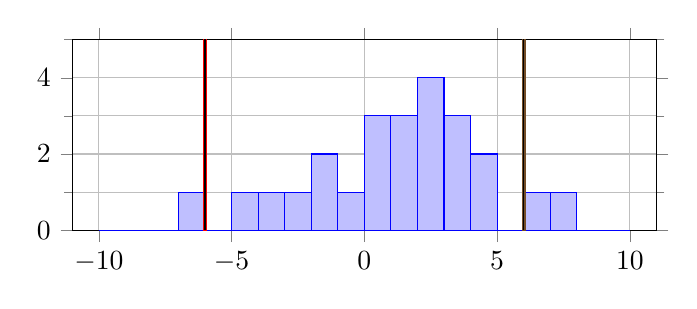
\begin{tikzpicture}
\begin{axis}[
height=4cm,
width=9cm,
%            ybar interval,      % <-- this causes the `xticks' to be centered
ymin= 0, ymax=5,
xmin=-11, xmax=11,
grid=both,
minor y tick num=1,
%yminorgrids=true,
tick align=outside, % <-- this positions the ticks "outside"
]
\addplot+ [
ybar interval,
mark=none,
fill=blue!25,   % fill the bars again
] coordinates {

	(-10,0)	%
	(-9,0)	%
	(-8,0)	%
	(-7,1)	%
	(-6,0)	%1
	(-5,1)	%11
	(-4,1)	%1
	(-3,1)	%111111
	(-2,2)	%1111
	(-1,1)	%11111
	 (0,3)	%111
	 (1,3)	%1
	 (2,4)	%
	 (3,3)	%
	 (4,2)	%
	 (5,0)	%
	 (6,1)	%
	 (7,1)	%
	 (8,0)	%
	 (9,0)	%
	 (10,1)	%

};

\addplot+ [
ybar interval,
mark=none,
fill=black,   % fill the bars again
] coordinates {
	(-6.05,16) 
	(-5.95,16) 
};

\addplot+ [
ybar interval,
mark=none,
fill=black,   % fill the bars again
] coordinates {
	(6.05,16) 
	(5.95,16) 
};
\end{axis}

\end{tikzpicture}
	\caption{Histogram of one sensor face reading the same tag multiple times. The Boundary lines represents tags that will not be read correctly.}
	\label{fig:histogram}
\end{figure}


%%%%%%%%%%%%%%%%%%%%%%%%%%%%%%%%%%%%%%%%%%%%%%%%%%%%%%%%%%%%%%%%%%%%%%%%%%%%%%%%%%%%%%%%%%%%%%%%%%%%%%%%%%%%%%%%%%%%%%%%%%%%%%%%%%%%%%%%%%%%%%
%%%%%%%%%%%%%%%%%%%%%%%%%%%%%%%%%%%%%%%%%%%%%%%%%%%%%%%%%%%%%%%%%%%%%%%%%%%%%%%%%%%%%%%%%%%%%%%%%%%%%%%%%%%%%%%%%%%%%%%%%%%%%%%%%%%%%%%%%%%%%%
%\begin{figure}[h]
%	\begin{tikzpicture}
\begin{axis}[view={-20}{20}, grid=both]
\addplot3[surf] file {data.txt};
\end{axis}
\end{tikzpicture}
       
%	\caption{Figure showing the error in the reading from a reader reading a tag as it is moved in X and Y relative to perfect alignment.}
%	\label{fig:histogram}
%\end{figure}
%%%%%%%%%%%%%%%%%%%%%%%%%%%%%%%%%%%%%%%%%%%%%%%%%%%%%%%%%%%%%%%%%%%%%%%%%%%%%%%%%%%%%%%%%%%%%%%%%%%%%%%%%%%%%%%%%%%%%%%%%%%%%%%%%%%%%%%%%%%%%%
%%%%%%%%%%%%%%%%%%%%%%%%%%%%%%%%%%%%%%%%%%%%%%%%%%%%%%%%%%%%%%%%%%%%%%%%%%%%%%%%%%%%%%%%%%%%%%%%%%%%%%%%%%%%%%%%%%%%%%%%%%%%%%%%%%%%%%%%%%%%%%

\section{Algorithims}
\label{sec:Algorithims}

This section describes two different algorhtims... These algorithims are similar to those described in...

\begin{algorithm}[htbp]
\hrulefill
\caption{Crystalization Algorithim}
\label{alg1}
\hrulefill
\begin{algorithmic}
\REQUIRE $n \geq 0$
\ENSURE $y = x^n$ 
\STATE $y \leftarrow 1$
\STATE $X \leftarrow x$
\STATE $N \leftarrow n$
 \WHILE{$N \neq 0$}
 \IF{$N$ is even}
\STATE $X \leftarrow X \times X$
\STATE $N \leftarrow N / 2$
\ELSE[$N$ is odd]
 \STATE $y \leftarrow y \times X$
\STATE $N \leftarrow N - 1$
\ENDIF
\ENDWHILE
\end{algorithmic}
\hrulefill
\end{algorithm}

\section{Experiments}
\label{sec:Experiments}

These experiments were implemented on a set of 12 Modified 3D M-Block modules. The control system which is running the experiments is described in Figure~\ref{fig:electroncsChart}.

\begin{figure}[ht]

	%% Figure of electronics Diagram
\tikzset{box/.style={draw, rectangle, rounded corners, thick, node distance=7em, text width=6em, text centered, minimum height=3.5em}}
\tikzset{container/.style={draw, rectangle, rounded corners, dashed, inner sep=1em}}
\tikzset{line/.style={draw, thick, -latex'}}

\begin{tikzpicture}[auto]
	\node[anchor=south west,inner sep=0, minimum width = \linewidth, minimum height = 8.5cm] (emptyBox) at (0,0) {};
	\begin{scope}[x={(emptyBox.south east)},y={(emptyBox.north west)}]
	\tikzset{>=latex}
		\coordinate (leftCenter) at (0.12, 0.75);
		\coordinate (rightCenter) at (0.6, 0.85);
		\coordinate (routePt) at (0.50, 0.75);
		
		% Main Board
		\node [box] (mainBoard) at (leftCenter) {High Level Control Board (ESP8266)};
		
		% Kyles Boards...
	%	\node [box] at ([shift = ({225:3.5 cm})] mainBoard) (kb) {Motor and Power Board (nRF51422)};
	%	\node [box, right = 1.5cm of kb] (db)  {Actuator Control Board};
		
		% Face Boards
		\node [box] (f0) at (rightCenter) {Face 0 PCB  (IO~Expander)};
		\node [box, below = 0.25cm of f0] (f1) {Face 1 PCB   (IO~Expander)};
		\node [below = 0.75cm of f1] (f2) {...};
		\node [box, below = 0.75cm of f2] (f5) {Face 5 PCB   (IO~Expander)};
		
		%% I2C Connections
		\path [line, <->, orange, ultra thick] (mainBoard) -- (routePt)-- (f0);
		\path [line, <->, orange, ultra thick] (mainBoard) -- (routePt)-- (f1);
		\path [line, <->, orange, ultra thick] (mainBoard) -- (routePt)-- (f5);
		
	%	\path [line, <->, orange, ultra thick] (kb) -- (db);
		
		%% Serial Connections
		
	%	\path [line, <->, blue, ultra thick] (kb) -- (mainBoard);

		%% Inputs
		\node [align = center] (input1) at (0.91, 0.45) {Environmental \\ and \\ Neighbor \\ sensing};
	%	\node [align = left] (input2) at (0.16, 0.96) {wifi commands};

	%	\node [align = left] (input3) at (0.25, 0.24) {Motor \\ Batteries \\ SMA wire};
	%	\node [align = left] (input4) at (0.4, 0.24) {Brake \\ Em coil};
		
%		\draw [dashed,  <->] (kb.south) to [out = 270, in = 180] (input3.west);
%		\draw [dashed,  <->] (input2.south) to [out = 270, in = 235] (mainBoard.west);
%		\draw [dashed,  <->] (input4.east) to [out = 0, in = 325] (db.east);
		
		\draw [dashed,  ->] (input1.north) to [out = 90, in = 0] (f0.east);
		\draw [dashed,  ->] (input1.north) to [out = 90, in = 0] (f1.east);
		\draw [dashed,  ->] (input1.south) to [out = 270, in = 0] (f5.east);
		
		% Dashed Boxes
	%	\node[container, fit = (mainBoard) (kb) (db) (input4) (input3)] (core) {};
	%	\node at (core.south) [below, node distance = 0 and 0] {\textbf{Core}};

		\node[container, fit = (f0) (f5)] (frame) {};
		\node at (frame.south) [below, node distance = 0 and 0] {\textbf{Frame}};

%    	\node [box] (planning) {Planning};
%   	 	\node [box, below of=planning, maroon, inner sep = 0pt] (resources) {Resources};
%   	 	\node [box, below of=resources] (sensors) {Sensors};
%    	\node [box, below of=sensors] (processing) {Processing};
%    	\node [box, below of=sensors] (processing) {Processing};
%    	\node [box, below of=sensors] (processing) {Processing};
%
%    	\coordinate (middle) at ($(resources.west)!0.5!(sensors.west)$);
%    	\node [box, above of=middle, node distance=4 cm] (archive) {Archive};
%    	\node [box, below of=archive, node distance=4 cm] (reporting) {Reporting};
%
%    	\node[container, fit=(resources) (sensors)] (or) {};
%    	\node at (or.north west) [above right,node distance=0 and 0] {OR};
%
%	    \node[container, fit=(archive) (reporting)] (his) {};
%    	\node at (his.north west) [above right,node distance=0 and 0] {HIS};
%
%    	\path [line, line width = 0.5mm, red] (planning) -- (resources);
%    	\path [line] (resources) -- (sensors);
%    	\path [line] (sensors) -- (processing);
%
%    	\path [line] (archive) |- (planning);
%    	\path [line] (archive) |- (processing);
%    	\path [line] (processing)--($(processing.south)-(0,0.5)$) -| (reporting);
%
%    	\draw [line] ($(processing.south)-(0,0.5)$) -- ++(4,0) node(lowerright){} |- (planning.east);
%    	\draw [line] (lowerright |- or.east) -- (or.east -| resources.south east);
%
%    	\draw[line] (archive.170)--(reporting.10);
%    	\draw[line] (reporting.350)--(archive.190);
    \end{scope}
\end{tikzpicture}


%
%
%	\begin{tikzpicture}
%	\node[anchor=south west,inner sep=0] (image) at (0,0) {\includegraphics[width=0.9\textwidth]{some_image.jpg}};
%	\begin{scope}[x={(image.south east)},y={(image.north west)}]
%
%	\end{scope}
%	\end{tikzpicture}
%\end{document}
	
\caption{This figure illustrates the various avenues of information exchange between the different elements of the experimental setup. The \emph{orange} arrows represent bi-directional WIFI messages sent between the immobile \emph{Server Module} and the active modules, with the dashed line showing a potentially faulty connection. The \emph{blue} arrows show the simple light-based messages which active modules are able to send to neighbors that they are directly connected to. The \emph{purple} arrows represent the reading of \tagNamePlural~ between an active module and a valid and adjacently connected \tagName. Note that \tagNamePlural can be read from both passive modules, and from passive or even unresponsive modules.}
	
	\label{fig:electroncsChart}
\end{figure}



%%%%%%%%%%%%%%%%%%%%%%%%%%%%%%%%%%%%%%%%%%%%%%%%%%%%%%%%%%%%%%%%%%%%%%%%%%%%%%%%%%%%%%%%%%%%%%%%%%%%%%%%%%%%%%%%%%%%%%%%%%%%%%%%%%%%%%%%%%%%%%%
%%%%%%%%%%%%%%%%%%%%%%%%%%%%%%%%%%%%%%%%%%%%%%%%%%%%%%%%%%%%%%%%%%%%%%%%%%%%%%%%%%%%%%%%%%%%%%%%%%%%%%%%%%%%%%%%%%%%%%%%%%%%%%%%%%%%%%%%%%%%%%%
\subsection{Arrow Following experiments}
\label{sec:mblocksExperimentsArrow}
%%%%%%%%%%%%%%%%%%%%%%%%%%%%%%%%%%%%%%%%%%%%%%%%%%%%%%%%%%%%%%%%%%%%%%%%%%%%%%%%%%%%%%%%%%%%%%%%%%%%%%%%%%%%%%%%%%%%%%%%%%%%%%%%%%%%%%%%%%%%%%%
%%%%%%%%%%%%%%%%%%%%%%%%%%%%%%%%%%%%%%%%%%%%%%%%%%%%%%%%%%%%%%%%%%%%%%%%%%%%%%%%%%%%%%%%%%%%%%%%%%%%%%%%%%%%%%%%%%%%%%%%%%%%%%%%%%%%%%%%%%%%%%%
We performed two set of experiments involving, the first involving only reading passive non-unique "arrow" tags, and the second including the
"virtual" or "stigmergic" arrows utilizing the globally unique connector faces embedded in active modules.

\begin{table}[h]
	\caption{Experimental results for }
	
	\begin{tabular}{ p{3.4cm}  p{1.9cm}  p{1.9cm} }
		\hline
								& Attempts 	& Successes \\
		\hline
		Configuration Discovery	&  -1 		& -50 \\
		Direction Following		& 0 		& 0  \\
		command Tags 			&  -1 		& -50 \\		
	\end{tabular}
	
	\label{tab:info}
\end{table}

\begin{figure}[h]  
	\centering
	\begin{subfigure}[b]{0.48\linewidth}
		\includegraphics[width=0.95\linewidth]{figures/arrows1.png}
		\subcaption{} 
	\end{subfigure}
	\begin{subfigure}[b]{0.48\linewidth}
		\includegraphics[width=0.95\linewidth]{figures/arrows2.png}
		\subcaption{} 
	\end{subfigure}
	
	\begin{subfigure}[b]{0.48\linewidth}
		\includegraphics[width=0.95\linewidth]{figures/arrows3.png}
		\subcaption{} 
	\end{subfigure}
	\begin{subfigure}[b]{0.48\linewidth}
		\includegraphics[width=0.95\linewidth]{figures/arrows4.png}
		\subcaption{} 
	\end{subfigure}
	
	\caption{This experiment the cube following a very simple embedded arrow path.}
	
	\label{fig:arrowExperiment}
\end{figure}

%%%%%%%%%%%%%%%%%%%%%%%%%%%%%%%%%%%%%%%%%%%%%%%%%%%%%%%%%%%%%%%%%%%%%%%%%%%%%%%%%%%%%%%%%%%%%%%%%%%%%%%%%%%%%%%%%%%%%%%%%%%%%%%%%%%%%%%%%%%%%%%
%%%%%%%%%%%%%%%%%%%%%%%%%%%%%%%%%%%%%%%%%%%%%%%%%%%%%%%%%%%%%%%%%%%%%%%%%%%%%%%%%%%%%%%%%%%%%%%%%%%%%%%%%%%%%%%%%%%%%%%%%%%%%%%%%%%%%%%%%%%%%%%
\subsection{line formation experiments}
\label{sec:mblocksExperimentsLine}
%%%%%%%%%%%%%%%%%%%%%%%%%%%%%%%%%%%%%%%%%%%%%%%%%%%%%%%%%%%%%%%%%%%%%%%%%%%%%%%%%%%%%%%%%%%%%%%%%%%%%%%%%%%%%%%%%%%%%%%%%%%%%%%%%%%%%%%%%%%%%%%
%%%%%%%%%%%%%%%%%%%%%%%%%%%%%%%%%%%%%%%%%%%%%%%%%%%%%%%%%%%%%%%%%%%%%%%%%%%%%%%%%%%%%%%%%%%%%%%%%%%%%%%%%%%%%%%%%%%%%%%%%%%%%%%%%%%%%%%%%%%%%%%

\begin{figure}[h]  
	\centering
	\begin{subfigure}[b]{0.32\linewidth}
		\includegraphics[width=0.95\linewidth]{figures/ActualLine_1.png}
		\subcaption{} 
	\end{subfigure}
	\begin{subfigure}[b]{0.32\linewidth}
		\includegraphics[width=0.95\linewidth]{figures/ActualLine_2.png}
		\subcaption{} 
	\end{subfigure}
	\begin{subfigure}[b]{0.32\linewidth}
		\includegraphics[width=0.95\linewidth]{figures/ActualLine_3.png}
		\subcaption{} 
	\end{subfigure}

	\begin{subfigure}[b]{0.32\linewidth}
		\includegraphics[width=0.95\linewidth]{figures/ActualLine_4.png}
		\subcaption{} 
	\end{subfigure}
	\begin{subfigure}[b]{0.32\linewidth}
		\includegraphics[width=0.95\linewidth]{figures/ActualLine_5.png}
		\subcaption{} 
	\end{subfigure}
	\begin{subfigure}[b]{0.32\linewidth}
		\includegraphics[width=0.95\linewidth]{figures/ActualLine_6.png}
		\subcaption{} 
	\end{subfigure}
	
	\caption{This experiment shows a random 3D configuration of M-Blocks reconfiguring into a line.}
	
	\label{fig:lineExperiment}
\end{figure}

These experiments involved several attempts to convert arbitrary generated 3D structures with a few constraints (no holes, and no modules connected by three or more connection faces) into a single horizontal line involving between 8 and 12 modules.

%%%%%%%%%%%%%%%%%%%%%%%%%%%%%%%%%%%%%%%%%%%%%%%%%%%%%%%%%%%%%%%%%%%%%%%%%%%%%%%%%%%%%%%%%%%%%%%%%%%%%%%%%%%%%%%%%%%%%%%%%%%%%%%%%%%%%%%%%%%%%%%
%%%%%%%%%%%%%%%%%%%%%%%%%%%%%%%%%%%%%%%%%%%%%%%%%%%%%%%%%%%%%%%%%%%%%%%%%%%%%%%%%%%%%%%%%%%%%%%%%%%%%%%%%%%%%%%%%%%%%%%%%%%%%%%%%%%%%

%%%%%%%%%%
\subsection{Light guided aggregation experiments}
\label{sec:mblocksExperimentsLight}
%%%%%%%%%%%%%%%%%%%%%%%%%%%%%%%%%%%%%%%%%%%%%%%%%%%%%%%%%%%%%%%%%%%%%%%%%%%%%%%%%%%%%%%%%%%%%%%%%%%%%%%%%%%%%%%%%%%%%%%%%%%%%%%%%%%%%%%%%%%%%%%
%%%%%%%%%%%%%%%%%%%%%%%%%%%%%%%%%%%%%%%%%%%%%%%%%%%%%%%%%%%%%%%%%%%%%%%%%%%%%%%%%%%%%%%%%%%%%%%%%%%%%%%%%%%%%%%%%%%%%%%%%%%%%%%%%%%%%%%%%%%%%%%

\begin{figure}[h]  
	\centering
	\begin{subfigure}[b]{0.48\linewidth}
		
		\begin{tikzpicture}[]	
			\node[opacity = 0.95] at (0,0) {\includegraphics[width = \linewidth]{figures/1-000.png}};
			\node[opacity = 0.5, fill = white, rounded corners] at (-1,-0.75) {t = 000 s};
		\end{tikzpicture}

	%	\subcaption{} 
	\end{subfigure}
	\begin{subfigure}[b]{0.48\linewidth}
		
		\begin{tikzpicture}[]	
		\node[opacity = 0.95] at (0,0) {\includegraphics[width = \linewidth]{figures/2-120.png}};
		\node[opacity = 0.5, fill = white, rounded corners] at (-1,-0.75) {t = 120 s};
		\end{tikzpicture}
		
	\end{subfigure}

	\begin{subfigure}[b]{0.48\linewidth}

		\begin{tikzpicture}[]	
		\node[opacity = 0.95] at (0,0) {\includegraphics[width = \linewidth]{figures/3-220.png}};
		\node[opacity = 0.5, fill = white, rounded corners] at (-1,-0.75) {t = 220 s};
		\end{tikzpicture}
		
	\end{subfigure}
	\begin{subfigure}[b]{0.48\linewidth}
		\begin{tikzpicture}[]	
		\node[opacity = 0.95] at (0,0) {\includegraphics[width = \linewidth]{figures/4-320.png}};
		\node[opacity = 0.5, fill = white, rounded corners] at (-1,-0.75) {t = 320 s};
		\end{tikzpicture}
	%	\subcaption{} 
	\end{subfigure}

	\begin{subfigure}[b]{0.48\linewidth}
		\begin{tikzpicture}[]	
		\node[opacity = 0.95] at (0,0) {\includegraphics[width = \linewidth]{figures/5-500.png}};
		\node[opacity = 0.5, fill = white, rounded corners] at (-1,-0.75) {t = 500 s};
		\end{tikzpicture} 
	\end{subfigure}
	\begin{subfigure}[b]{0.48\linewidth}
		\begin{tikzpicture}[]	
		\node[opacity = 0.95] at (0,0) {\includegraphics[width = \linewidth]{figures/6-600.png}};
		\node[opacity = 0.5, fill = white, rounded corners] at (-1,-0.75) {t = 600 s};
		\end{tikzpicture}
	\end{subfigure}
	
	\caption{This experiment shows a random 3D tracking light.}
	
	\label{fig:LightExperiment}
\end{figure}

These experiments essentially attempt to implement the photo-taxis Braitenberg behavior for a group of M-Blocks modules. There is a single light source, and a special target module, which when modules aggregate to it, the modules share its location through wireless and light signals for additional modules to connect to it - essentially forming a single "crystal" of aggregated modules. In these experiment modules are gradually released into a confined (0.5m x 0.5 m) bounded foam-padded location, and move until they either run out of battery or connect to the designated aggregate.


%%%%%%%%%%%%%%%%%%%%%%%%%
\section{Introduction}
\label{sec:Introduction}
%%%%%%%%%%%%%%%%%%%%%%%%%

We did things... Things are good. Bye!


%%% TESTING THINGS WITH the tikz
%\begin{tikzpicture}
%\begin{scope}
%
%\newcounter{xa}
%\newcounter{ya}
%\newcounter{za}
%
%% The angles of x,y,z-axes
%\newcommand\xaxisa{210}
%\newcommand\yaxisa{-30}
%\newcommand\zaxisa{90}
%
%\newcommand\leftsidea[3]{
%	\fill[fill=red, draw=black,shift={(\xaxisa:#1)},shift={(\yaxisa:#2)},
%	shift={(\zaxisa:#3)}] (0,0) -- (0,-1) -- (210:1) --(150:1)--(0,0);
%}


%leftsidea{1}{1}{1};
%\end{scope}
%\end{tikzpicture}


%%%%%%%%%%%%%%%%%%%%%%%%%
\section*{Acknowledgments}
This work is supported by the NSF through grants 1240383 and 1138967.
%%%%%%%%%%%%%%%%%%%%%%%%% 
\section*{Supplementary Material}
\url{http://youtu.be/y27gUFO6mTA}

\bibliographystyle{IEEEtran}

\bibliography{RomanishinMamishRus-ICRA18.bib}


\end{document}
